% =====================================================================
%  DetailHOI --- Human Skeletal Priors for Positional Query Refinement
%  in Human-Object Interaction Detection
%
%  Journal-submission format (single column, double-ish spaced, continuous
%  line numbers, Elsevier-style front/back matter), matching the companion
%  VideoHOI manuscript template.
%
%  Self-contained: compiles with any standard TeX distribution
%  (pdflatex detailhoi.tex, twice, for cross-references).
%  Figures expected in ./figures/ as PDF.
% =====================================================================
\documentclass[12pt,a4paper]{article}

\usepackage[margin=2.5cm]{geometry}
\usepackage[T1]{fontenc}
\usepackage[utf8]{inputenc}
\usepackage{mathptmx} % Times-like text and math font
\usepackage{amsmath,amssymb,bm}
\usepackage{graphicx}
\usepackage{booktabs}
\usepackage{multirow}
\usepackage{caption}
\usepackage{subcaption}
\usepackage{microtype}
\usepackage{xcolor}
\usepackage{setspace}
\usepackage[right]{lineno}
\usepackage[colorlinks,linkcolor=black,citecolor=black,urlcolor=blue!60!black]{hyperref}

\captionsetup{font=small,labelfont=bf,skip=5pt}
\setlength{\abovecaptionskip}{6pt}
\setlength{\belowcaptionskip}{2pt}

\newcommand{\bx}{\mathbf{b}}
\newcommand{\bc}{\mathbf{c}}
\newcommand{\be}{\mathbf{e}}
\newcommand{\bp}{\mathbf{p}}
\newcommand{\bq}{\mathbf{q}}
\newcommand{\bz}{\mathbf{z}}
\newcommand{\PE}{\mathrm{PE}}
\newcommand{\R}{\mathbb{R}}

\title{\bfseries DetailHOI: Human Skeletal Priors for Positional\\
Query Refinement in Human--Object Interaction Detection}

\author{%
{\large Chunyu Jiang$^{a,\ast}$, Chao Chen$^{a}$, Michael Yu Wang$^{a}$}\\[6pt]
{\normalsize $^{a}$Department of Mechanical and Aerospace Engineering, Monash University, Clayton, VIC 3800, Australia}\\[12pt]
{\footnotesize $^\ast$Corresponding author.}\\[2pt]
{\footnotesize E-mail addresses: \texttt{reginaldjcy@gmail.com} (C.~Jiang), [e-mail] (C.~Chen), [e-mail] (M.Y.~Wang).}\\[2pt]
{\footnotesize ORCID: [ORCID] (C.~Jiang); [ORCID] (C.~Chen); [ORCID] (M.Y.~Wang).}\\[10pt]
{\footnotesize\itshape Declarations of interest: none.}
}
\date{}

\begin{document}
\onehalfspacing
\maketitle
\linenumbers

% =====================================================================
\begin{abstract}
Human--Object Interaction (HOI) detection localises people and objects and names
the action that binds them, producing triplets of the form
$\langle$\emph{human}, \emph{action}, \emph{object}$\rangle$. The strongest and
most training-efficient detectors are two-stage transformers built on a frozen
DETR, in which a learnable interaction query attends over image features under
the guidance of a \emph{positional} query derived from the detected boxes. That
positional query treats a person exactly as it treats a chair: a centre and a
size. We argue this discards the single most informative signal a two-stage
detector already has access to for free---the geometry of the human body itself.

We present \textbf{DetailHOI}, which re-expresses the human half of the
interaction query's positional embedding in the body's own coordinate frame. A
frozen top-down pose estimator supplies $K$ skeletal keypoints per detected
person; each keypoint receives a sinusoidal positional embedding, the stack is
modulated by a learned, content-conditioned estimate of the skeleton's spatial
extent, and a single linear map compresses it into the $D_h$ dimensions
previously occupied by the human box centre. The object half is compressed into
the remaining $D_o = 512 - D_h$ dimensions. The change is confined to the
construction of the positional query: the detector, the decoder, the loss and
the inference cost of the pipeline are untouched, and it adds $1.77$M parameters
($0.6\%$ of the model).

On V-COCO and HICO-DET, DetailHOI improves over a PViC baseline trained under
identical settings, reaching $71.42$ mAP on V-COCO and $33.74$ mAP on HICO-DET
against $71.28$ and $33.35$ respectively, with the gain concentrated on
non-rare classes ($34.77 \rightarrow 35.39$). Our ablations report a result we
believe is more useful than the headline: \emph{denser skeletons are worse}.
Interpolating additional points along the skeleton graph ($K = 23$, $K = 31$)
costs accuracy relative to the $17$ native COCO joints, and how the fixed
$512$-dimensional positional budget is \emph{split} between the human and the
object matters as much as what is put into it.
\end{abstract}

% =====================================================================
\section{Introduction}
\label{sec:intro}

Human--Object Interaction detection asks a model to go beyond naming the objects
in a scene and to state how a person is engaging with them. The output is a set
of triplets $\langle$\emph{human}, \emph{action}, \emph{object}$\rangle$, each
grounded by a pair of boxes. The task underpins a wide range of downstream
systems---collaborative robotics, driver and pedestrian intent modelling,
surveillance analytics, and augmented-reality assistants---because knowing
\emph{that} a person and a cup are co-present is far less useful than knowing
that the person is about to \emph{drink} from it.

Progress on the task has been rapid but uneven. Two obstacles dominate. The
first is the extreme long tail of interaction categories: HICO-DET's $600$
interaction classes follow a distribution in which a large fraction of classes
are observed a handful of times. The second is spatial ambiguity. A single
image may contain several people and a dozen objects; the number of candidate
pairs grows quadratically, and most of them are not interacting at all. A
detector that cannot decide \emph{which} object a given person is oriented
towards will spend its capacity discriminating actions for pairs that should
never have been scored.

Transformer-based detectors address the second problem with attention. The
DETR family~\cite{carion2020detr} recast detection as set prediction over
learnable queries, and HOI detectors inherited the idea, either end-to-end
\cite{tamura2021qpic,kim2021hotr,zou2021hoitrans} or in a two-stage form that
reuses a frozen detector and learns only an interaction head
\cite{zhang2022upt,zhang2023pvic}. The two-stage route has proven both more
accurate and dramatically cheaper to train, and the reason is now well
understood: a query that starts from an \emph{explicit spatial anchor}
converges far faster than one initialised at random, an observation first made
for object detection~\cite{meng2021conditional,liu2022dabdetr} and then carried
into HOI detection by PViC~\cite{zhang2023pvic}. In PViC, each interaction query
is paired with a positional query built from the two boxes of the candidate
pair: sinusoidal embeddings of the human box centre and the object box centre
are concatenated and used as the query-side positional term in cross-attention,
so the query is told \emph{where to look} before it has learned \emph{what to
look for}.

\paragraph{The gap.} That positional query is object-centric in a literal
sense---it is built from box geometry, and a box is the same primitive whether
it contains a person or a fire hydrant. Yet the human in an HOI triplet is not
an interchangeable box. Its pose is a structured, low-dimensional signal that
already encodes the reachable workspace of the hands, the direction the torso
faces, and the stage of the action being performed. Two people whose boxes are
identical can be reaching in opposite directions. A positional prior that
collapses a person to a centre point throws that information away at exactly
the moment it would be most useful: when the query is deciding which region of
the feature map to attend to.

\paragraph{Our approach.} We keep everything about the two-stage recipe and
change one component. For every detected person we obtain $K$ skeletal
keypoints from a frozen, off-the-shelf top-down pose estimator, embed each
keypoint with the same sinusoidal function the baseline applies to box centres,
modulate the stack by a learned estimate of the skeleton's own spatial extent
(the pose analogue of the box-size modulation used in
DAB-DETR~\cite{liu2022dabdetr} and PViC), and project the result into the
$D_h$ dimensions that the human box centre used to occupy. The object retains
the remaining $D_o = 512 - D_h$. The positional query therefore carries a
\emph{posture} on the human side and a \emph{location} on the object side,
within an unchanged budget and an unchanged decoder. Figure~\ref{fig:flow}
reproduces the pipeline as presented in the candidature review;
\S\ref{sec:method} gives the notation-precise version of what is actually
implemented and evaluated.

\begin{figure}[t]
\centering
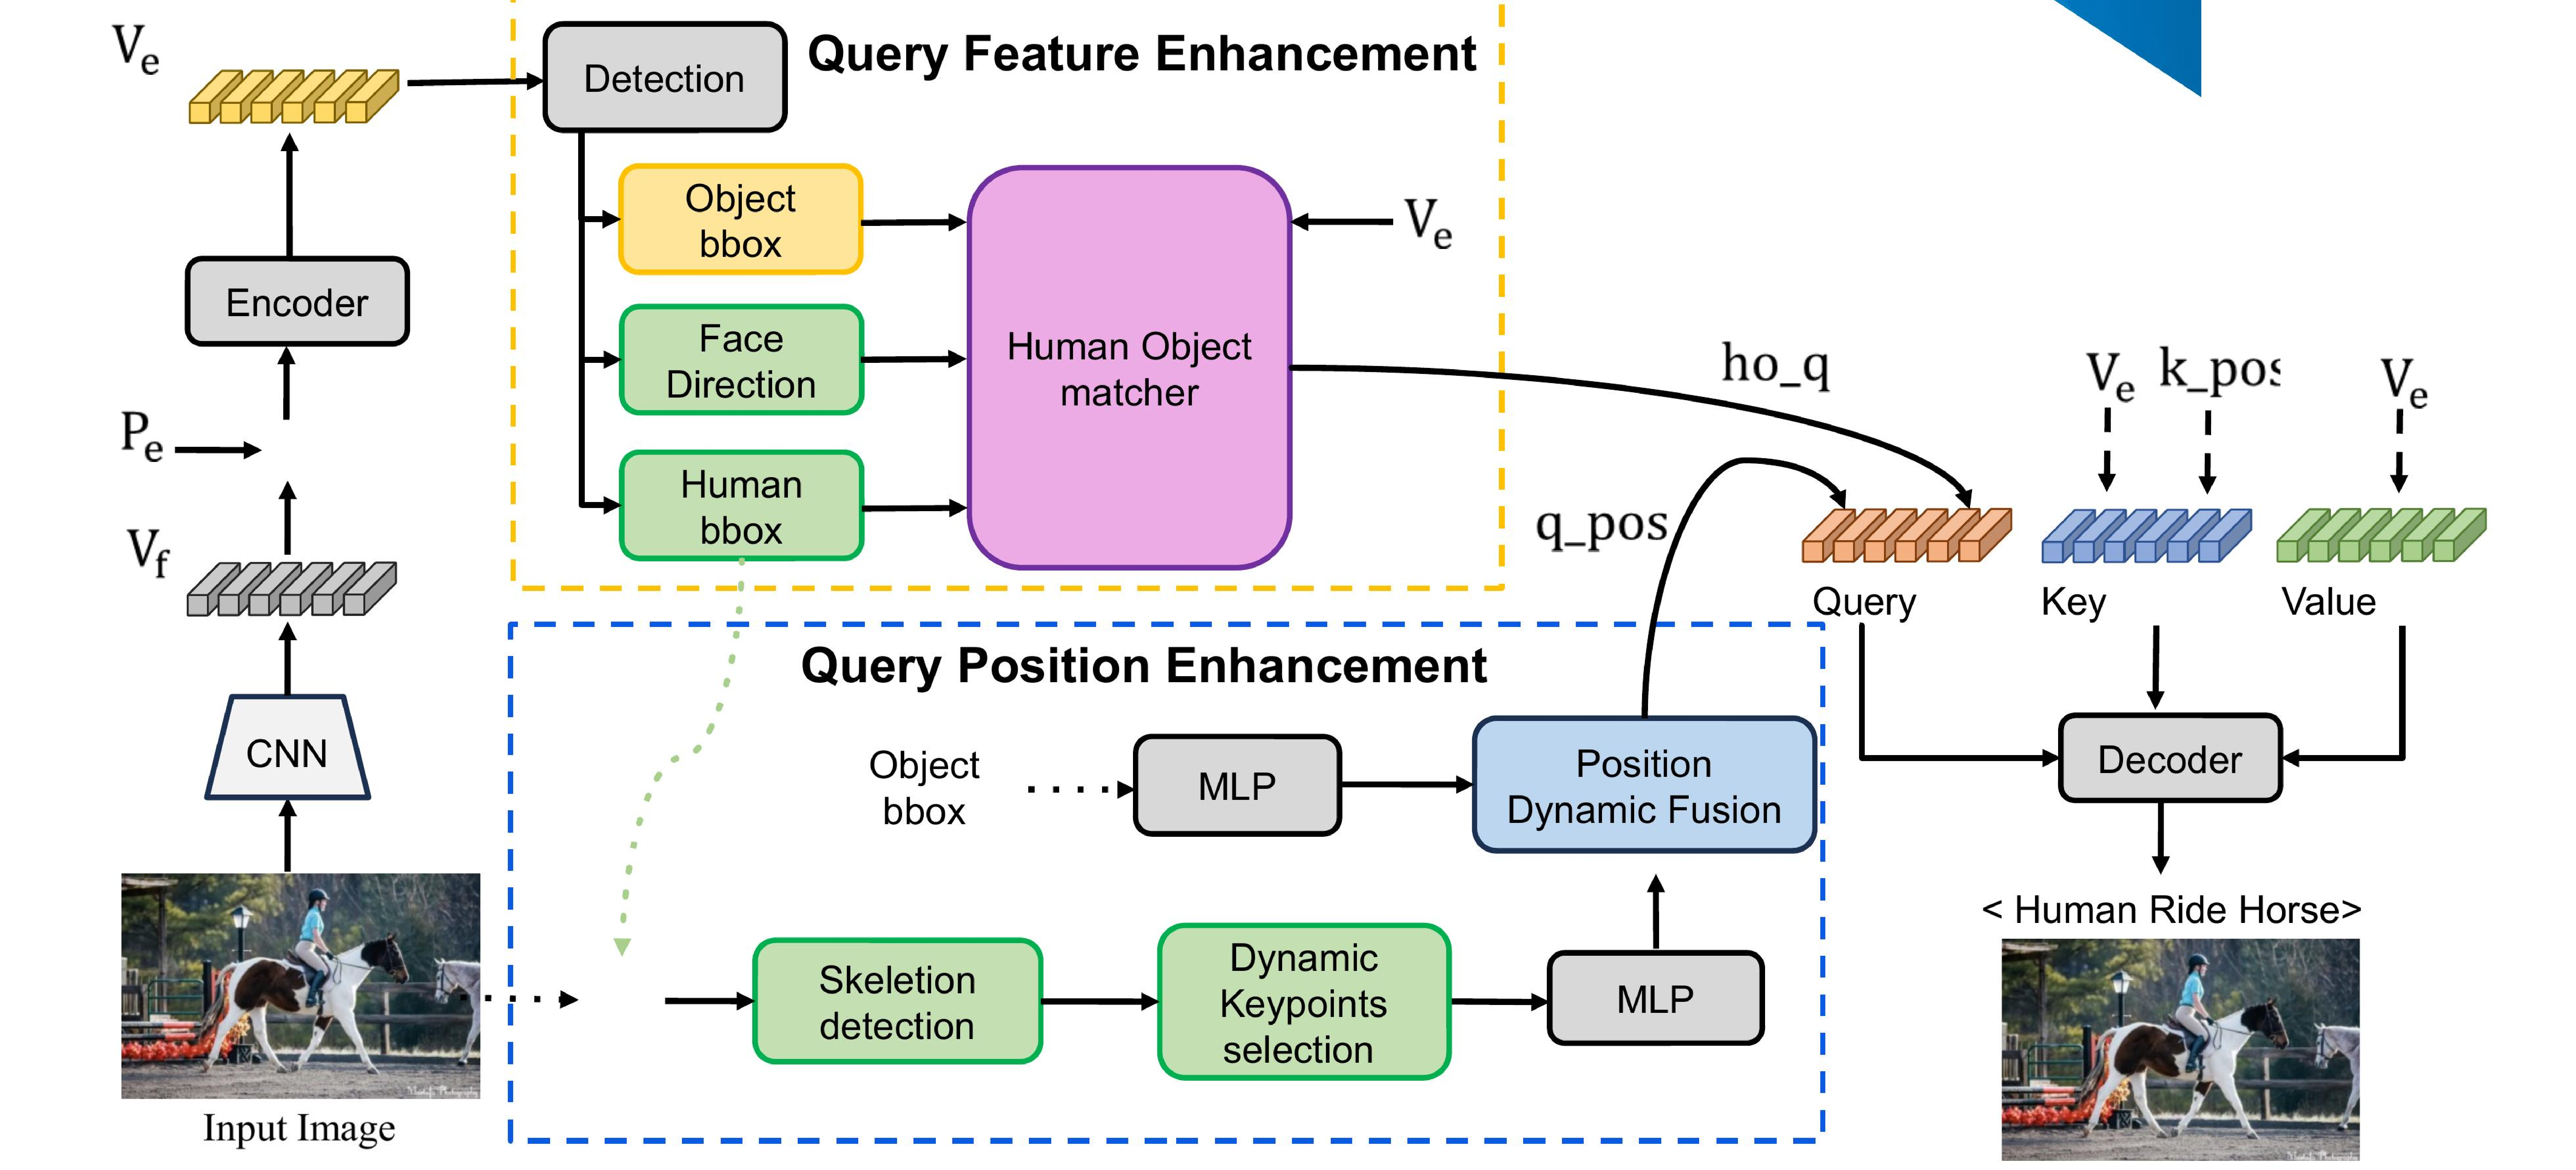
\includegraphics[width=\textwidth]{figures/flowchart.pdf}
\caption{\textbf{Pipeline flow chart}, reproduced from the candidature-review
presentation. A frozen CNN/encoder produces global image features $V_e$
(positionally encoded by $P_e$); detection yields object and human boxes. The
\emph{Query Feature Enhancement} branch (top) combines the object box, the
human box and $V_e$ through a Human--Object matcher into the content query
\texttt{ho\_q}. The \emph{Query Position Enhancement} branch (bottom) runs
skeleton detection and dynamic keypoint selection on the human box, fuses this
with the object box through an MLP and a Position Dynamic Fusion module into
the positional query \texttt{q\_pos}. Query, key ($V_e$ with \texttt{k\_pos})
and value ($V_e$) feed a shared decoder that outputs the interaction triplet.
\textbf{Two things this figure shows that the evaluated system does not
have:} the \emph{Face Direction} input to the matcher is the head-orientation
extension discussed as future work in \S\ref{sec:discussion} and is not part
of any result in this paper; and the input/output photographs are the
presentation's own examples, credited ``Mustafa Photography''---that credit
is not yet cleared for publication and must be resolved (author permission or
a licensed substitute) before submission.}
\label{fig:flow}
\end{figure}

\paragraph{Contributions.}
\begin{enumerate}\itemsep1pt\parskip0pt
\item \textbf{Skeleton-conditioned positional query refinement.} We replace the
human half of the interaction query's positional embedding with a
confidence-aware, extent-modulated embedding of the human skeleton. The
modification is local, adds $1.77$M parameters ($\approx 0.6\%$), and leaves
the detector, decoder, loss and inference schedule untouched
(\S\ref{sec:method}).
\item \textbf{An asymmetric positional budget.} Because the human and object
halves of the positional query no longer carry the same kind of information,
there is no reason for them to be the same size. We treat the split
$(D_h, D_o)$ as a design variable and show it matters: $384/128$ beats
$256/256$ under an identical keypoint set (\S\ref{sec:ablation}).
\item \textbf{A negative result on skeletal density.} We densify the skeleton by
interpolating points along the COCO skeleton graph, reaching $K=23$ and $K=31$.
Both are \emph{worse} than the $17$ native joints. Interpolated points are
deterministic functions of the joints they lie between; they add parameters and
dilute the projection without adding information (\S\ref{sec:ablation}).
\item \textbf{A human-clarity evaluation protocol.} We isolate the subset of
each benchmark in which instances are large and unambiguous enough for pose
estimation to be reliable, and report a controlled comparison on it, which
separates the merit of the prior from the noise of the pose estimator
(\S\ref{sec:filtering}, \S\ref{sec:ablation}).
\end{enumerate}

% =====================================================================
\section{Related Work}
\label{sec:related}

\subsection{Two-stage and one-stage HOI detection}
Early HOI detectors were two-stage by necessity: an off-the-shelf detector such
as Faster R-CNN~\cite{ren2015faster} produced instances, and a second network
classified the interaction for each human--object pair
\cite{gkioxari2018interactnet,li2019tin,gupta2019nofrills}. The design is
modular but pays a quadratic cost in the number of instances and suffers from a
representational mismatch: features optimised for object identity are not
necessarily the features that discriminate \emph{verbs}.

One-stage transformer detectors removed the pairing bottleneck by predicting
triplets directly from a set of learnable queries
\cite{tamura2021qpic,kim2021hotr,zou2021hoitrans}. They are elegant and fast at
inference, but they inherit DETR's slow convergence and typically require long
schedules.

The current strongest configuration is a hybrid: keep a \emph{frozen}
pretrained DETR as the instance source and train only a lightweight interaction
head. UPT~\cite{zhang2022upt} showed that unary and pairwise representations of
the frozen detector's own decoder embeddings are sufficient to reach
competitive accuracy at a fraction of the training cost.
PViC~\cite{zhang2023pvic} added a small cross-attention decoder that lets each
pair query re-read the backbone feature map, with box-derived positional
embeddings steering where it reads. Our work sits squarely in this line and
modifies precisely the steering signal.

\subsection{What a query is, and why its prior matters}
In DETR~\cite{carion2020detr}, a query is a learnable slot that interacts with
image features through cross-attention,
\begin{equation}
\mathrm{Attn}(Q,K,V) = \mathrm{softmax}\!\left(\frac{QK^{\!\top}}{\sqrt{d_k}}\right)V ,
\end{equation}
and decodes one object hypothesis. The original formulation initialises those
slots randomly, with no spatial meaning, and needs on the order of $500$ epochs
to converge. The remedy discovered independently by several groups is to give
each query an explicit positional identity: Conditional
DETR~\cite{meng2021conditional} decouples content from spatial attention;
DAB-DETR~\cite{liu2022dabdetr} makes the query a literal 4-D anchor box and
modulates its positional embedding by the anchor's width and height;
Deformable DETR~\cite{zhu2021deformable} restricts attention to a learned set
of offsets around a reference point. All three share the same insight: a query
that knows where it is converges much faster than one that does not.

PViC~\cite{zhang2023pvic} transplants this into HOI detection. Each candidate
pair $(i,j)$ carries a positional query
$[\PE(\bc_i); \PE(\bc_j)] \in \R^{512}$ built from the two box centres, plus a
box-level term used in the query self-attention. The paper shows that this
anchoring lets the decoder ``pin-point'' body parts and auxiliary objects
relevant to the verb. Our contribution is to observe that the human half of
this pair of anchors is describing the wrong object: the person, unlike the
object, has an internal structure that a single point cannot represent.

\subsection{Priors in HOI detection}
Prior knowledge has been injected into HOI detectors from three directions.
\emph{Spatial} priors encode the relative geometry of the two boxes---centre
offsets, aspect ratios, intersection-over-union---and are typically appended to
the pair representation~\cite{zhang2021scg,zhang2022upt}. \emph{Semantic}
priors import knowledge from vision--language models such as
CLIP~\cite{radford2021clip} to transfer to rare and unseen compositions
\cite{liao2022genvlkt,ning2023hoiclip,cao2023unihoi}. \emph{Structural} priors
model the scene as a graph and reason over it~\cite{zhang2021scg}. More recent
work has explored 3-D and attentional priors: HORP~\cite{liu2023horp} adds 3-D
location cues to resolve depth ambiguity in 2-D images together with a
text-expressed ``gaze area'' cue, and generative approaches such as
VRDiff~\cite{vrdiff} learn dense visual relation representations. What these
share is a focus on the object or the scene; the human is treated as one more
detected entity.

\subsection{Human-centric and pose-aware modelling}
A parallel line of work has long argued that pose is the natural prior for HOI.
PMFNet~\cite{wan2019pmfnet} routes attention through pose-aware multi-level
features; TIN~\cite{li2019tin} learns a transferable notion of
``interactiveness'' partly from human appearance; pose-attention networks such
as PAIN~\cite{pain} and geometric--visual graph models such as
GeoVis-GNN~\cite{geovisgnn} combine skeletal keypoints with object geometry
through graph convolutions. Beyond the body, gaze is a strong leading indicator
of intent, and recent work estimates it from head orientation in egocentric and
hand--object settings~\cite{hoigaze,hagi}.

Almost all of this work injects pose into the \emph{content} pathway---as extra
features to be fused, or as nodes in a graph. Our proposal is different and,
we think, simpler: pose enters the \emph{positional} pathway, replacing the
anchor that tells the query where to attend, and never touches the content
representation at all. This keeps the interaction head's feature dimensionality,
parameter count and runtime essentially unchanged, and it makes the ablations
interpretable, because any change in accuracy is attributable to the geometry of
attention rather than to added representational capacity.

% =====================================================================
\section{Method}
\label{sec:method}

\begin{figure}[t]
\centering
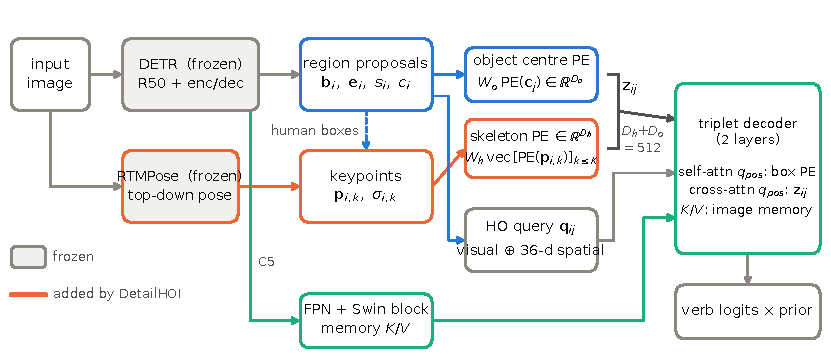
\includegraphics[width=\textwidth]{figures/architecture.pdf}
\caption{\textbf{DetailHOI.} The detector and the pose estimator are frozen;
only the interaction head is trained. The path drawn in orange is what we add.
Instead of embedding the human box centre, we embed all $K$ keypoints of the
detected skeleton, modulate the stack by a content-conditioned estimate of the
skeleton's spatial extent, and compress it to $D_h$ dimensions. The object
centre is compressed to $D_o = 512 - D_h$. Their concatenation $\bz_{ij}$ is the
positional query of the decoder's cross-attention---the same slot, the same
width, and the same decoder as the baseline.}
\label{fig:arch}
\end{figure}

\subsection{Preliminaries: positional queries in a two-stage detector}
\label{sec:prelim}

A frozen DETR produces, for image $I$, a set of instances
$\{(\bx_i, c_i, s_i, \be_i)\}_{i=1}^{N}$: a box, a category, a score and the
$256$-dimensional decoder embedding that generated it. Instances are ordered so
that the $N_h$ humans precede the objects. Every ordered pair $(i,j)$ with
$i < N_h$ and $i \neq j$ becomes a candidate interaction.

Let $\bc_i \in [0,1]^2$ be the normalised centre of $\bx_i$ and
$(w_i, h_i)$ its normalised size. Let $\PE : \R^2 \to \R^{256}$ be the
sinusoidal embedding that maps a 2-D point to a $256$-vector by stacking the
$128$-dimensional codes of its two coordinates. The baseline builds a centre
embedding $\mathbf{u}_i$, a size embedding $\mathbf{v}_i$ and their
concatenation,
\begin{equation}
\mathbf{u}_i = \PE(\bc_i), \quad
\mathbf{v}_i = \PE\big((w_i,h_i)\big), \quad
\mathbf{g}_i = [\,\mathbf{u}_i ; \mathbf{v}_i\,] \in \R^{512},
\end{equation}
and modulates the centre term by a content-conditioned reference size,
following DAB-DETR. Writing $\mathbf{u}^{y}_i$ and $\mathbf{u}^{x}_i$ for the
first and second halves of $\mathbf{u}_i$,
\begin{equation}
(r^w_i, r^h_i) = \sigma\big(\mathrm{MLP}_{\text{anc}}(\be_i)\big), \quad
\mathbf{u}^{y}_i \leftarrow \tfrac{r^h_i}{h_i}\,\mathbf{u}^{y}_i, \quad
\mathbf{u}^{x}_i \leftarrow \tfrac{r^w_i}{w_i}\,\mathbf{u}^{x}_i .
\label{eq:boxmod}
\end{equation}
The interaction query itself is a content vector
$\bq_{ij} \in \R^{384}$ produced by fusing the pair's visual embeddings with a
$36$-dimensional hand-crafted spatial encoding of the two boxes. The decoder
then runs $L=2$ layers of self-attention over queries followed by
cross-attention into a Swin-processed backbone feature map, with two positional
terms:
\begin{equation}
\bz^{\text{box}}_{ij} = [\,\mathbf{g}_i ; \mathbf{g}_j\,] \in \R^{1024},
\qquad
\bz_{ij} = [\,\mathbf{u}_i ; \mathbf{u}_j\,] \in \R^{512},
\label{eq:baselinez}
\end{equation}
the former added to queries and keys in self-attention, the latter concatenated
head-wise to the query in cross-attention. Equation~\eqref{eq:baselinez} is the
object of this paper: $\bz_{ij}$ is the signal that decides \emph{where} each
pair query reads the image, and its first half describes a person by a single
point.

\paragraph{Why the positional term is the right place to intervene.}
Cross-attention with additive positional encodings is a sum of four terms, a
decomposition made explicit by Conditional DETR~\cite{meng2021conditional}.
Writing $\mathbf{k}_\ell$ for the content key at memory location $\ell$ and
$\mathbf{k}^{\text{pos}}_\ell$ for its positional encoding, the pre-softmax
score for pair query $(i,j)$ expands as
\begin{equation}
\mathrm{score}_{ij,\ell} \;\propto\;
\underbrace{\bq_{ij}\!\cdot\!\mathbf{k}_\ell^{\top}}_{\text{content--content}}
\;+\;
\underbrace{\bq_{ij}\!\cdot\!\mathbf{k}^{\text{pos}\top}_\ell}_{\text{content--position}}
\;+\;
\underbrace{\bz_{ij}\!\cdot\!\mathbf{k}_\ell^{\top}}_{\text{position--content}}
\;+\;
\underbrace{\bz_{ij}\!\cdot\!\mathbf{k}^{\text{pos}\top}_\ell}_{\text{position--position}}.
\label{eq:decomp}
\end{equation}
The content query $\bq_{ij}$ is untouched by this paper, and so is the
content--position term, which depends on $\bq_{ij}$ alone. Replacing the human
half of $\bz_{ij}$ therefore acts only on the position--content and
position--position terms: it changes which locations a pair query prefers
\emph{a priori}, not what the query recognises once it attends there. This is
the formal statement of the claim we return to in
\S\ref{sec:discussion}---the mechanism is geometric, not semantic, by
construction.

\subsection{Skeleton-conditioned positional embedding}
\label{sec:skeleton}

\paragraph{Keypoints.} For each detected human box we run a frozen top-down
pose estimator (RTMPose-L~\cite{jiang2023rtmpose}, a SimCC-style
model~\cite{li2022simcc} trained on COCO) and obtain $K$ keypoints
$\bp_{i,k} \in \R^2$ with confidences $\sigma_{i,k} \in [0,1]$. Object
instances receive an all-zero keypoint tensor and are never used on the human
side of a pair. Detection and pose estimation are both performed under
\texttt{no\_grad}: no gradient flows into either frozen module, so the pose
estimator is a fixed feature extractor, not a jointly-trained branch.

\paragraph{Per-keypoint embedding.} Each keypoint is normalised by the image
size and embedded with the \emph{same} sinusoidal function the baseline applies
to box centres,
\begin{equation}
\PE(\bp_{i,k}) \in \R^{256}, \qquad k = 1, \dots, K .
\end{equation}
Reusing $\PE$ is deliberate: it keeps the human and object halves of the
positional query in a common frequency basis, so the decoder's positional
projection does not have to reconcile two unrelated encodings.

\paragraph{Extent modulation.} Equation~\eqref{eq:boxmod} rescales the box
centre embedding by the box's own size, which makes the embedding's effective
frequency adapt to how large the instance is. The skeleton needs the same
treatment, but its natural scale is not the box---a seated person and a standing
person with the same box height have very different joint spreads. We therefore
compute the extent of the \emph{confident} joints,
\begin{equation}
(\hat{w}_i, \hat{h}_i) =
\max_{k \in \mathcal{V}_i} \bp_{i,k} - \min_{k \in \mathcal{V}_i} \bp_{i,k},
\qquad
\mathcal{V}_i = \{k : \sigma_{i,k} > \tau\},
\end{equation}
with $\tau = 0.3$, falling back to $(1,1)$ when no joint is confident, and
modulate against a learned reference derived from the instance's own content
embedding:
\begin{equation}
(s^w_i, s^h_i) = \sigma\big(\mathrm{MLP}_{\text{kpt}}(\be_i)\big),\quad
\mathbf{m}^{y}_{i,k} \leftarrow \tfrac{s^h_i}{\hat{h}_i}\,\mathbf{m}^{y}_{i,k},
\quad
\mathbf{m}^{x}_{i,k} \leftarrow \tfrac{s^w_i}{\hat{w}_i}\,\mathbf{m}^{x}_{i,k},
\end{equation}
where $\mathbf{m}_{i,k} = \PE(\bp_{i,k})$ and the superscripts again denote its
two halves.
This is the mechanism by which the confidence scores enter the model. They are
not used as a soft mask over keypoints---they define which joints are allowed
to set the skeleton's scale, so that a spurious low-confidence ankle in the
corner of the crop cannot stretch the whole embedding.

\paragraph{Compression.} The modulated stack is flattened and projected by a
single linear map $W_h \in \R^{D_h \times 256K}$:
\begin{equation}
\mathbf{h}_i = W_h \,\mathrm{vec}\big([\mathbf{m}_{i,1}; \dots; \mathbf{m}_{i,K}]\big)
\in \R^{D_h}.
\end{equation}
The object side is compressed by $W_o \in \R^{D_o \times 256}$ applied to the
modulated box-centre embedding,
$\mathbf{o}_j = W_o\, \mathbf{u}_j \in \R^{D_o}$, and the positional query of
the cross-attention becomes
\begin{equation}
\boxed{\;\bz_{ij} = [\,\mathbf{h}_i \,;\, \mathbf{o}_j\,] \in \R^{512},
\qquad D_h + D_o = 512 .\;}
\label{eq:ours}
\end{equation}
Comparing~\eqref{eq:ours} with~\eqref{eq:baselinez}: the width is identical, the
consumer is identical, and the self-attention term $\bz^{\text{box}}_{ij}$ is
left exactly as the baseline defines it. Only the semantics of the first
$D_h$ dimensions have changed---from ``the person is here'' to ``the person is
shaped like this, here.''

\subsection{The positional budget is a design variable}
\label{sec:budget}

The baseline splits its $512$ positional dimensions evenly by construction:
$256$ for the human centre, $256$ for the object centre, because both are
$\PE$ outputs. Once the human half carries a $K$-joint skeleton and the object
half carries a single point, symmetry is no longer justified---the two halves
have very different intrinsic dimensionality. We therefore treat $(D_h, D_o)$
as a hyper-parameter subject to $D_h + D_o = 512$, and evaluate $384/128$
against $256/256$ in \S\ref{sec:ablation}---shorthand \emph{ratio3} and
\emph{ratio1} below, after the multiple of $128$ each gives the human half.
This is a free variable in the sense that changing it does not change the
decoder, the query width, or the number of attention heads; it only
re-partitions a vector that already exists. At the sparse end of $K$ the split
need not even be a multiple of $128$: Table~\ref{tab:params}'s $K{=}6$ row uses
a \emph{variable} split ($439/73$) chosen by the same criterion, more of the
budget than either fixed ratio would give a six-joint skeleton.

\subsection{Skeletal density: interpolating the skeleton graph}
\label{sec:density}

If $17$ joints help, do more points help further? The COCO skeleton defines a
graph over the $17$ joints---four torso edges, four arm edges, four leg edges
and two neck edges, $E = 14$ in total. We densify by placing $m$ evenly-spaced
points along each edge,
\begin{equation}
\bp^{(t)}_{i,(u,v)} = (1-t)\,\bp_{i,u} + t\,\bp_{i,v},
\quad t = \tfrac{1}{m+1},\dots,\tfrac{m}{m+1},
\end{equation}
assigning each interpolated point the confidence
$\min(\sigma_{i,u}, \sigma_{i,v})$ so that a limb with one unreliable endpoint
does not inject confident-looking phantom points. With $m=1$ this yields
$K = 17 + 14 = 31$. We also evaluate a lighter variant that interpolates only
the six most action-relevant edges (upper arms, thighs, and the shoulder and
hip lines), giving $K = 23$, and two coarse variants at the opposite end:
$K = 6$ (head centroid, both wrists, both ankles, torso centre) and $K = 3$
(head centroid and the two wrists). Section~\ref{sec:ablation} reports what
happens.

\subsection{Cost}
\label{sec:cost}

Table~\ref{tab:params} lists the parameters introduced by
Eq.~\eqref{eq:ours}. The dominant term is $W_h$, whose size grows linearly in
$K$. At our default setting ($K{=}17$, $D_h{=}384$) the head grows by
$1.77$M parameters, about $0.6\%$ of the full pipeline, and no term scales with
image resolution or with the number of candidate pairs. The frozen pose
estimator adds one forward pass per image over the detected human crops; because
it is frozen and batched per image, it does not enter the backward pass at all.

\begin{table}[t]
\centering\small
\setlength{\tabcolsep}{4.5pt}
\begin{tabular}{lrrr}
\toprule
Configuration & $W_h$ & $W_o$ + $\mathrm{MLP}_{\text{kpt}}$ & Total \\
\midrule
$K{=}3$,\quad $256/256$  & \phantom{0}0.20\,M & 0.13\,M & 0.33\,M \\
$K{=}6$,\quad $439/73$   & \phantom{0}0.67\,M & 0.09\,M & 0.76\,M \\
$K{=}17$, $256/256$   & \phantom{0}1.11\,M & 0.13\,M & 1.25\,M \\
\textbf{$K{=}17$, $384/128$} & \phantom{0}1.67\,M & 0.10\,M & \textbf{1.77\,M} \\
$K{=}23$, $256/256$   & \phantom{0}1.51\,M & 0.13\,M & 1.64\,M \\
$K{=}31$, $256/256$   & \phantom{0}2.03\,M & 0.13\,M & 2.16\,M \\
\bottomrule
\end{tabular}
\caption{Parameters added to the interaction head. $W_h$ dominates and grows
linearly in the number of keypoints $K$; nothing else in the model changes.}
\label{tab:params}
\end{table}

% =====================================================================
\section{Experimental Setup}
\label{sec:setup}

\subsection{Datasets}
\textbf{V-COCO}~\cite{gupta2015vcoco} is built on MS-COCO
2014~\cite{lin2014coco} and annotates $24$ action classes over $80$ object
categories. After discarding images without an annotated human--object pair we
use $4{,}969$ \texttt{trainval} images and $4{,}532$ \texttt{test} images.
\textbf{HICO-DET}~\cite{chao2018hicodet} is the larger and harder benchmark:
$38{,}118$ training and $9{,}658$ test images, $117$ verbs, $80$ objects and
$600$ interaction classes, with a standard partition into $138$ rare and $462$
non-rare classes.

\subsection{The human-clarity subset}
\label{sec:filtering}

A pose-based prior can only be as good as the pose. On both benchmarks a
substantial fraction of images contain people who are heavily occluded, motion
blurred, or a few dozen pixels tall---cases in which a top-down pose estimator
returns joints that are confidently wrong. Averaging over such images conflates
two questions: whether the skeletal prior helps, and how often the skeleton is
recoverable at all.

To separate them we construct a \emph{human-clarity subset} of each benchmark.
An off-the-shelf YOLOv8-n detector~\cite{yolov8} is run over every image and an
image is retained only if it yields at least one detection at confidence
$\geq 0.8$. This is a deliberately cheap, model-agnostic proxy for ``the
instances in this image are large and unambiguous''; it is not a person-specific
test, and we return to that limitation in \S\ref{sec:limitations}. The
resulting subsets are listed in Table~\ref{tab:data}. Roughly one image in eight
is removed from V-COCO and one in five from HICO-DET.

\begin{table}[t]
\centering\small
\setlength{\tabcolsep}{4pt}
\begin{tabular}{llrrr}
\toprule
Dataset & Split & All & Clear & Kept \\
\midrule
\multirow{2}{*}{V-COCO}
  & trainval  & 4{,}969  & 4{,}404  & 88.6\% \\
  & test      & 4{,}532  & 3{,}971  & 87.6\% \\
\midrule
\multirow{2}{*}{HICO-DET}
  & train2015 & 38{,}118 & 30{,}083 & 78.9\% \\
  & test2015  & \phantom{0}9{,}658  & \phantom{0}7{,}658  & 79.3\% \\
\bottomrule
\end{tabular}
\caption{The human-clarity subset. ``All'' counts images with at least one
annotated interaction; ``Clear'' counts those retained by the confidence filter
of \S\ref{sec:filtering}.}
\label{tab:data}
\end{table}

\subsection{Metrics}
We report mean average precision over interaction classes, with a detection
counted as correct when both boxes reach IoU $\geq 0.5$ with a ground-truth pair
and the interaction label matches. AP is computed with $11$-point interpolation.
On HICO-DET we report the standard full / rare / non-rare breakdown over the
$600$ interaction classes.

\paragraph{A note on the V-COCO protocol.} Our V-COCO numbers are produced by
the in-repository evaluator over the $24$ action classes, \emph{not} by the
official V-COCO \texttt{AP\textsubscript{role}} script. The two protocols differ
in how they handle the no-object actions and in their AP interpolation, and the
in-repository numbers run substantially higher. They are therefore valid for
\emph{comparing configurations trained and evaluated identically}, which is the
purpose they serve here, and are not comparable to published
\texttt{AP\textsubscript{role}} figures. All V-COCO comparisons in this paper
are internal.

\subsection{Implementation details}
The instance detector is DETR-R50~\cite{carion2020detr} fine-tuned on the
respective dataset and frozen throughout. Region proposals are kept above a
score of $0.05$, with between $3$ and $15$ instances per image. Pose comes from
frozen RTMPose-L at $256 \times 192$, run top-down on the detected human boxes,
so keypoints are associated with their proposals by construction. The interaction head uses a query width of
$384$, one Swin encoder block over the C5 feature map, and a two-layer triplet
decoder with $8$ heads and dropout $0.1$. Training uses
AdamW~\cite{loshchilov2019adamw} with learning rate $10^{-4}$, weight decay
$10^{-4}$, batch size $92$ over two RTX A6000 GPUs (DDP, world size $2$), for
$30$ epochs with the learning rate dropped by $0.2\times$ at epoch $20$. The
classification loss is a binary focal loss~\cite{lin2017focal} with
$\alpha = 0.5$, $\gamma = 0.1$, combined multiplicatively with the detector's
prior scores raised to $\lambda = 2.8$. The random seed is fixed at $140$. One
V-COCO epoch takes approximately $19$ minutes in this configuration.

% =====================================================================
\section{Results}
\label{sec:results}

\subsection{Main comparison}

Table~\ref{tab:main} compares DetailHOI at its default setting ($K{=}17$,
$D_h/D_o = 384/128$) against the PViC baseline trained under identical settings.
On V-COCO the skeletal prior improves the internal mAP from $71.28$ to $71.42$.
On HICO-DET it improves full mAP from $33.35$ to $33.74$, an increase of $0.39$
points.

The breakdown is more informative than the aggregate. The gain is carried
entirely by the non-rare classes, $34.77 \rightarrow 35.39$ ($+0.62$), while
rare classes decline slightly, $28.59 \rightarrow 28.23$ ($-0.36$). This is
what one should expect from a \emph{geometric} prior rather than a semantic one.
A skeleton tells the decoder where to look; it says nothing about what a rarely
seen verb looks like. Classes with enough examples to learn an
attention-to-verb mapping benefit; classes seen a handful of times do not have
enough signal to exploit a sharper attention pattern, and pay the small cost of
a positional query whose object half has been compressed from $256$ to $128$
dimensions. Methods that improve the rare split do so by importing external
semantics~\cite{liao2022genvlkt,ning2023hoiclip,cao2023unihoi}; that is an
orthogonal and complementary axis to ours.

\begin{table}[t]
\centering\small
\setlength{\tabcolsep}{4pt}
\begin{tabular}{lcccc}
\toprule
& V-COCO$^{\dagger}$ & \multicolumn{3}{c}{HICO-DET} \\
\cmidrule(lr){2-2}\cmidrule(lr){3-5}
Configuration & mAP & Full & Rare & Non-rare \\
\midrule
PViC baseline                     & 71.28 & 33.35 & \textbf{28.59} & 34.77 \\
\textbf{DetailHOI} ($K{=}17$)     & \textbf{71.42} & \textbf{33.74} & 28.23 & \textbf{35.39} \\
\quad + human-clarity training set & 71.33 & 33.51 & 28.79 & 34.92 \\
\bottomrule
\end{tabular}
\caption{Main results at epoch $30$, identical schedules throughout.
$^{\dagger}$V-COCO numbers use the in-repository diagnostic evaluator and are
internally comparable only (\S\ref{sec:setup}). The skeletal prior helps the
aggregate and the non-rare split; it does not help rare classes.}
\label{tab:main}
\end{table}

\subsection{Ablations on the human-clarity subset}
\label{sec:ablation}

The main comparison mixes the effect of the prior with the frequency of images
in which pose is unreliable. To isolate the prior we retrain every configuration
on the human-clarity subset of V-COCO and evaluate on its test split, so that
every model sees only images in which the skeleton is recoverable.
Figure~\ref{fig:conv} shows the training curves and Table~\ref{tab:ablation}
the final numbers.

\begin{figure}[t]
\centering
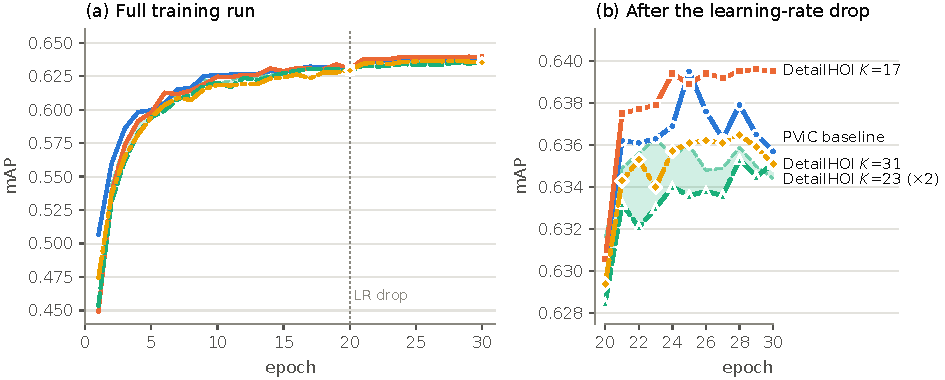
\includegraphics[width=\linewidth]{figures/convergence.pdf}
\caption{Convergence on the human-clarity subset of V-COCO. All configurations
share a schedule; the learning-rate drop at epoch $20$ is marked. Panel (b)
magnifies the post-drop region where the configurations separate. Denser
skeletons ($K{=}23$, $K{=}31$) sit consistently below both the baseline and
$K{=}17$ for the whole of the second phase---the ordering is stable, not a
single-epoch fluctuation.}
\label{fig:conv}
\end{figure}

\begin{table}[t]
\centering\small
\setlength{\tabcolsep}{4pt}
\begin{tabular}{lccc}
\toprule
Configuration & $D_h/D_o$ & Best & Epoch 30 \\
\midrule
PViC baseline (no keypoints)      & 256/256 & 63.95 & 63.57 \\
\textbf{$K{=}17$ COCO joints}     & \textbf{384/128} & \textbf{63.96} & \textbf{63.95} \\
$K{=}23$ interpolated             & 256/256 & 63.63 & 63.44 \\
$K{=}31$ interpolated             & 256/256 & 63.65 & 63.51 \\
\bottomrule
\end{tabular}
\caption{Keypoint granularity and positional budget, V-COCO human-clarity
subset. All rows are trained and evaluated on the same subset under the same
schedule. The two interpolated skeletons are clearly worse; the $17$ native
joints with an asymmetric budget are best, and are markedly more stable across
the final ten epochs.}
\label{tab:ablation}
\end{table}

\begin{figure}[t]
\centering
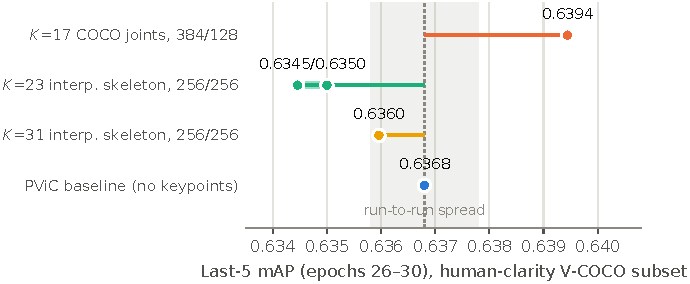
\includegraphics[width=\linewidth]{figures/ablation.pdf}
\caption{Best subset mAP per configuration, relative to the baseline (dashed).
Adding interpolated points along the skeleton graph costs roughly $0.3$ mAP.}
\label{fig:ablation}
\end{figure}

\paragraph{Denser skeletons are worse.} $K{=}23$ and $K{=}31$ both land around
$63.6$, roughly $0.3$ points below the $17$-joint model and below the baseline.
We think the reason is structural rather than a tuning artefact. An interpolated
point is an exact convex combination of two joints that are already in the
stack, so it carries no information the projection did not already have. What it
does carry is cost: $W_h$ grows from $1.67$M to $2.03$M parameters, the
sinusoidal stack is diluted by redundant rows, and the extent statistic
$(\hat{w}, \hat{h})$ is computed over a set whose interior is now densely
populated, making it less sensitive to the extremities that actually define
reach. The lesson generalises beyond this architecture: when a prior is
compressed by a single linear map, adding deterministic functions of existing
inputs is not free.

\paragraph{The budget split matters.} The $K{=}17$ model runs at $384/128$ and
the interpolated models at $256/256$; the $17$-joint configuration is the only
one that gives the human side more than half the positional budget, and it is
the only one that improves on the baseline. This is consistent with the
intuition that a $K$-joint skeleton has genuinely more spatial degrees of
freedom than a single point and needs more room to survive compression, while
the object's centre needs very little---$128$ dimensions of a $256$-dimensional
sinusoidal code are apparently enough to localise a box centre. We regard the
split as a first-class hyper-parameter of this design rather than an
implementation detail.

\paragraph{Stability, not just peak.} The final-epoch column of
Table~\ref{tab:ablation} is worth reading alongside the best column. The
baseline peaks at $63.95$ but ends at $63.57$, oscillating by nearly $0.4$
points over the last ten epochs (Fig.~\ref{fig:conv}b). DetailHOI peaks at
$63.96$ and ends at $63.95$. On the peak metric the two are tied; on the
end-of-schedule metric---the one that matters if you are not selecting
checkpoints on the test set---the skeletal prior is worth $0.38$ points and
removes most of the late-training variance. A positional query anchored to a
stable body geometry appears to give the decoder a less noisy target than one
anchored to a box centre that shifts with every detector jitter.

\paragraph{Filtering as a training strategy.} Training on the human-clarity
subset and evaluating on the full benchmark (last row of Table~\ref{tab:main})
lands between the baseline and full DetailHOI on the aggregate, but is the best
of the three on rare classes ($28.79$). Removing noisy images helps precisely
where data is scarcest and a few corrupted examples do the most damage; it hurts
elsewhere, simply because $11\%$--$21\%$ of the training data is gone. Filtering
is therefore better understood as a diagnostic instrument---which is how we use
it in this section---than as a way to gain accuracy.

\subsection{Qualitative: what the positional term attends to}
\label{sec:qualitative}

Equation~\eqref{eq:decomp} splits the cross-attention score of a trained
DetailHOI model into four terms; Figure~\ref{fig:attn} renders each of them
separately for the same query on the same image, alongside the full score the
decoder actually uses. The content--content term (1) is diffuse--- it is the
same regardless of where any instance sits, so it lights up anything that
looks like the query's target class. The position--position term (2), built
purely from $\bz_{ij}$, is by contrast sharply concentrated on the annotated
human--object pair even with the content pathway switched off, which is the
qualitative counterpart of the claim in \S\ref{sec:discussion}: the skeletal
prior alone is informative about \emph{where} to look. The two cross terms (3,
4) are weaker than either diagonal term, and the full score (5) inherits its
spatial concentration mainly from term (2). This single-example view should
not be read as a quantitative claim, but it is consistent with the ablation
result above---on this query, the positional term is not a minor conditioning
signal but appears to be the dominant source of spatial selectivity in the
head.

\begin{figure}[t]
\centering
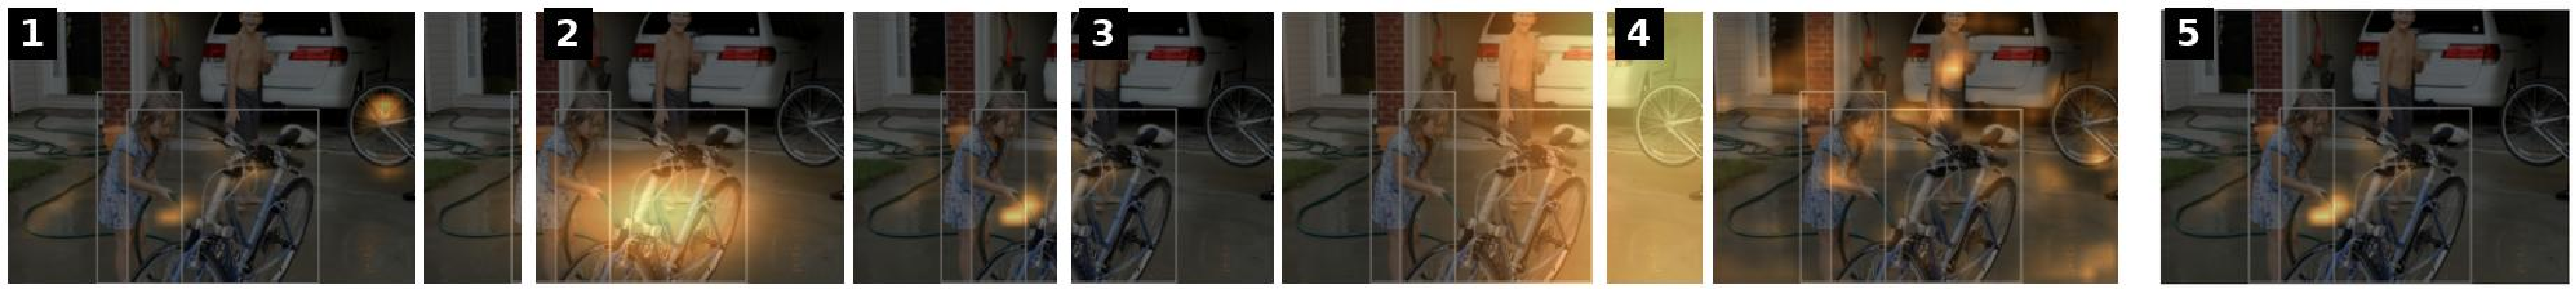
\includegraphics[width=\textwidth]{figures/attention.pdf}
\caption{\textbf{Decomposing the attention score.} Panels correspond to the
four terms of Eq.~\eqref{eq:decomp} for one human--object query---(1)
content--content $\bq_{ij}\!\cdot\!\mathbf{k}_\ell^\top$, (2)
position--position $\bz_{ij}\!\cdot\!\mathbf{k}^{\text{pos}\top}_\ell$, (3)
content--position $\bq_{ij}\!\cdot\!\mathbf{k}^{\text{pos}\top}_\ell$, (4)
position--content $\bz_{ij}\!\cdot\!\mathbf{k}_\ell^\top$---and (5) the full,
summed score the decoder attends with. Boxes mark the annotated human and
object.}
\label{fig:attn}
\end{figure}

\subsection{Context}

Table~\ref{tab:sota} places our numbers among published HICO-DET results.
Our baseline reproduces PViC at $33.35$ rather than the published $34.69$; the
gap is a training-budget difference, not a claim about the method---we train
for $30$ epochs at batch $92$ with a frozen detector and no schedule search,
whereas the published figure uses the authors' full recipe. The comparison that
carries weight in this paper is the internal one of Tables~\ref{tab:main}
and~\ref{tab:ablation}, where every row shares a schedule, a seed and an
evaluator.

\begin{table}[t]
\centering\small
\setlength{\tabcolsep}{4pt}
\begin{tabular}{llccc}
\toprule
Method & Backbone & Full & Rare & Non-rare \\
\midrule
QPIC~\cite{tamura2021qpic}       & R50 & 29.07 & 21.85 & 31.23 \\
UPT~\cite{zhang2022upt}          & R50 & 31.66 & 25.94 & 33.36 \\
PViC~\cite{zhang2023pvic}        & R50 & 34.69 & 32.14 & 35.45 \\
\midrule
PViC (our schedule)              & R50 & 33.35 & 28.59 & 34.77 \\
\textbf{DetailHOI} (ours)        & R50 & 33.74 & 28.23 & 35.39 \\
\bottomrule
\end{tabular}
\caption{HICO-DET in context. Rows above the rule are quoted from the
respective papers under their own training recipes; rows below share ours.}
\label{tab:sota}
\end{table}

% =====================================================================
\section{Discussion}
\label{sec:discussion}

\paragraph{What the result does and does not say.} The honest summary is that a
skeletal positional prior buys a small, consistent improvement---about $0.4$ mAP
on HICO-DET, concentrated on non-rare classes, plus a noticeable gain in
end-of-training stability---for $0.6\%$ more parameters and no change to the
decoder or the inference schedule. It is not a large gain, and on the
human-clarity subset the peak accuracy is a tie. What makes the result
interesting is where it comes from: not from adding features to the content
pathway, which is what pose-aware HOI models have traditionally done, but from
changing the geometry of attention while holding representational capacity
essentially fixed. That the change registers at all is evidence that the
positional query, not just the content query, is a productive place to inject
human structure.

\paragraph{Why interpolation fails, and what would not.} The density ablation
should not be read as ``more keypoints cannot help.'' It shows that
\emph{deterministic} elaborations of an existing keypoint set cannot help,
because a linear projection can already form any convex combination of its
inputs. Points that would carry new information---dense body-part segmentations,
contact points predicted by a separate model, or a 3-D lift of the
skeleton---are a different proposition, because they are not functions of the
$17$ joints.

\paragraph{Toward head-orientation priors.} The natural extension of this work,
and the one we originally set out to build, is to add head orientation and gaze
to the human half of the positional query. The architecture accommodates it
without modification: a head-pose feature would be projected and concatenated
into the same $D_h$ block that currently holds the skeleton, subject to the same
$D_h + D_o = 512$ budget, and would give the decoder an attentional direction
rather than only a body configuration---plausibly reaching interactions that
have not yet begun, which is exactly where a purely kinematic prior has nothing
to say. Related evidence from the gaze literature is
encouraging~\cite{hoigaze,hagi,liu2023horp}. We stress that this component is
\emph{not} part of the system evaluated here, and that no result in this paper
depends on it.

\subsection{Limitations}
\label{sec:limitations}

Three caveats bound the claims above.

\emph{The clarity filter is a proxy.} As implemented, the filter keeps an image
if any object is detected with confidence $\geq 0.8$, not specifically a person.
It correlates with image quality and instance scale, which is what we needed,
but a person-specific criterion---a minimum human box area, or a minimum mean
keypoint confidence---would isolate the intended variable more sharply. We
expect the qualitative conclusions to hold, since the failure modes it removes
(blur, extreme scale) are not person-specific, but the exact subset would
differ.

\emph{One seed, and one confounded baseline.} All ablations use a single seed
($140$). The margins in Table~\ref{tab:ablation} are a few tenths of a point,
which is the same order as the epoch-to-epoch oscillation visible in
Figure~\ref{fig:conv}b; the ordering is stable across the final ten epochs,
which is our evidence that it is real, but multi-seed variance is not measured.
Separately, the subset baseline was trained at batch size $64$ against $92$ for
the DetailHOI rows, a confound we did not control.

\emph{V-COCO numbers are internal.} As noted in \S\ref{sec:setup}, they come
from the diagnostic evaluator, not the official \texttt{AP\textsubscript{role}}
protocol, and should not be compared against published V-COCO figures.

% =====================================================================
\section{Conclusion}

We asked what happens if the positional prior of an interaction query stops
treating a person as a box. DetailHOI replaces the human half of that
prior---and only that half---with a confidence-aware, extent-modulated embedding
of the human skeleton, compressed into the same dimensions the box centre used
to occupy. The change costs $1.77$M parameters, touches neither the frozen
detector nor the decoder, and improves HICO-DET full mAP from $33.35$ to
$33.74$, with the gain concentrated on non-rare classes and a marked reduction
in late-training instability.

The ablations are the more transferable part of the result. Densifying the
skeleton by interpolating along its graph makes things \emph{worse}, because a
single linear projection can already form those combinations; and how the fixed
positional budget is split between the human and the object matters as much as
what is put into the human half. Both findings apply to any design that
compresses a structured prior into a positional query. The clearest next step is
to add a signal that is genuinely new rather than derived---head orientation
being the obvious candidate---within the same budget, and to test whether it
reaches the interactions a kinematic prior cannot see: the ones that have not
started yet.

% =====================================================================
\section*{CRediT authorship contribution statement}
\noindent Chunyu Jiang: Conceptualization, Methodology, Software, Validation,
Formal analysis, Investigation, Data curation, Visualization, Writing --
original draft. Chao Chen: Conceptualization, Methodology, Supervision,
Writing -- review \& editing, Funding acquisition. Michael Yu Wang:
Supervision, Resources, Writing -- review \& editing.

\section*{Declaration of competing interest}
\noindent The authors declare that they have no known competing financial
interests or personal relationships that could have appeared to influence the
work reported in this paper.

\section*{Declaration of generative AI and AI-assisted technologies in the writing process}
\noindent During the preparation of this work the authors used [tool name] in
order to [reason]. After using this tool, the authors reviewed and edited the
content as needed and take full responsibility for the content of the
published article.

\section*{Funding}
\noindent This research did not receive any specific grant from funding
agencies in the public, commercial, or not-for-profit sectors.

\section*{Data availability}
\noindent The V-COCO and HICO-DET datasets used in this study are publicly
available and remain subject to their original licences. The code, trained
checkpoints and evaluation logs supporting the findings of this study will be
made available at [repository URL] upon acceptance.

\section*{Acknowledgements}
\noindent [Acknowledgements, if any.]

% =====================================================================
{\small
% NOTE: entries marked [verify] are carried over from the project's earlier
% draft and their bibliographic details should be checked against the source
% before submission.
\begin{thebibliography}{99}\itemsep1pt

\bibitem{carion2020detr}
N.~Carion, F.~Massa, G.~Synnaeve, N.~Usunier, A.~Kirillov, and S.~Zagoruyko.
\newblock End-to-end object detection with transformers.
\newblock In \emph{ECCV}, 2020.

\bibitem{zhang2023pvic}
F.~Z. Zhang, Y.~Yuan, D.~Campbell, Z.~Zhong, and S.~Gould.
\newblock Exploring predicate visual context in detecting human--object interactions.
\newblock In \emph{ICCV}, 2023.

\bibitem{zhang2022upt}
F.~Z. Zhang, D.~Campbell, and S.~Gould.
\newblock Efficient two-stage detection of human--object interactions with a novel unary--pairwise transformer.
\newblock In \emph{CVPR}, 2022.

\bibitem{zhang2021scg}
F.~Z. Zhang, D.~Campbell, and S.~Gould.
\newblock Spatially conditioned graphs for detecting human--object interactions.
\newblock In \emph{ICCV}, 2021.

\bibitem{tamura2021qpic}
M.~Tamura, H.~Ohashi, and T.~Yoshinaga.
\newblock QPIC: Query-based pairwise human--object interaction detection with image-wide contextual information.
\newblock In \emph{CVPR}, 2021.

\bibitem{kim2021hotr}
B.~Kim, J.~Lee, J.~Kang, E.-S. Kim, and H.~J. Kim.
\newblock HOTR: End-to-end human--object interaction detection with transformers.
\newblock In \emph{CVPR}, 2021.

\bibitem{zou2021hoitrans}
C.~Zou, B.~Wang, Y.~Hu, J.~Liu, Q.~Wu, Y.~Zhao, B.~Li, C.~Zhang, C.~Zhang,
Y.~Wei, and J.~Sun.
\newblock End-to-end human object interaction detection with HOI transformer.
\newblock In \emph{CVPR}, 2021.

\bibitem{meng2021conditional}
D.~Meng, X.~Chen, Z.~Fan, G.~Zeng, H.~Li, Y.~Yuan, L.~Sun, and J.~Wang.
\newblock Conditional DETR for fast training convergence.
\newblock In \emph{ICCV}, 2021.

\bibitem{liu2022dabdetr}
S.~Liu, F.~Li, H.~Zhang, X.~Yang, X.~Qi, H.~Su, J.~Zhu, and L.~Zhang.
\newblock DAB-DETR: Dynamic anchor boxes are better queries for DETR.
\newblock In \emph{ICLR}, 2022.

\bibitem{zhu2021deformable}
X.~Zhu, W.~Su, L.~Lu, B.~Li, X.~Wang, and J.~Dai.
\newblock Deformable DETR: Deformable transformers for end-to-end object detection.
\newblock In \emph{ICLR}, 2021.

\bibitem{ren2015faster}
S.~Ren, K.~He, R.~Girshick, and J.~Sun.
\newblock Faster R-CNN: Towards real-time object detection with region proposal networks.
\newblock In \emph{NeurIPS}, 2015.

\bibitem{gkioxari2018interactnet}
G.~Gkioxari, R.~Girshick, P.~Doll\'{a}r, and K.~He.
\newblock Detecting and recognizing human--object interactions.
\newblock In \emph{CVPR}, 2018.

\bibitem{li2019tin}
Y.-L. Li, S.~Zhou, X.~Huang, L.~Xu, Z.~Ma, H.-S. Fang, Y.~Wang, and C.~Lu.
\newblock Transferable interactiveness knowledge for human--object interaction detection.
\newblock In \emph{CVPR}, 2019.

\bibitem{gupta2019nofrills}
T.~Gupta, A.~Schwing, and D.~Hoiem.
\newblock No-frills human--object interaction detection: Factorization, layout encodings, and training techniques.
\newblock In \emph{ICCV}, 2019.

\bibitem{wan2019pmfnet}
B.~Wan, D.~Zhou, Y.~Liu, R.~Li, and X.~He.
\newblock Pose-aware multi-level feature network for human object interaction detection.
\newblock In \emph{ICCV}, 2019.

\bibitem{liao2022genvlkt}
Y.~Liao, A.~Zhang, M.~Lu, Y.~Wang, X.~Li, and S.~Liu.
\newblock GEN-VLKT: Simplify association and enhance interaction understanding for HOI detection.
\newblock In \emph{CVPR}, 2022.

\bibitem{ning2023hoiclip}
S.~Ning, L.~Qiu, Y.~Liu, and X.~He.
\newblock HOICLIP: Efficient knowledge transfer for HOI detection with vision--language models.
\newblock In \emph{CVPR}, 2023.

\bibitem{cao2023unihoi}
Y.~Cao, Q.~Tang, X.~Su, C.~Song, S.~You, X.~Lu, and C.~Xu.
\newblock Detecting any human--object interaction relationship: Universal HOI detector with spatial prompt learning on foundation models.
\newblock In \emph{NeurIPS}, 2023.

\bibitem{radford2021clip}
A.~Radford, J.~W. Kim, C.~Hallacy, A.~Ramesh, G.~Goh, S.~Agarwal, G.~Sastry,
A.~Askell, P.~Mishkin, J.~Clark, G.~Krueger, and I.~Sutskever.
\newblock Learning transferable visual models from natural language supervision.
\newblock In \emph{ICML}, 2021.

\bibitem{jiang2023rtmpose}
T.~Jiang, P.~Lu, L.~Zhang, N.~Ma, R.~Han, C.~Lyu, Y.~Li, and K.~Chen.
\newblock RTMPose: Real-time multi-person pose estimation based on MMPose.
\newblock \emph{arXiv:2303.07399}, 2023.

\bibitem{li2022simcc}
Y.~Li, S.~Yang, P.~Liu, S.~Zhang, Y.~Wang, Z.~Wang, W.~Yang, and S.-T. Xia.
\newblock SimCC: A simple coordinate classification perspective for human pose estimation.
\newblock In \emph{ECCV}, 2022.

\bibitem{lin2014coco}
T.-Y. Lin, M.~Maire, S.~Belongie, J.~Hays, P.~Perona, D.~Ramanan,
P.~Doll\'{a}r, and C.~L. Zitnick.
\newblock Microsoft COCO: Common objects in context.
\newblock In \emph{ECCV}, 2014.

\bibitem{chao2018hicodet}
Y.-W. Chao, Y.~Liu, X.~Liu, H.~Zeng, and J.~Deng.
\newblock Learning to detect human--object interactions.
\newblock In \emph{WACV}, 2018.

\bibitem{gupta2015vcoco}
S.~Gupta and J.~Malik.
\newblock Visual semantic role labeling.
\newblock \emph{arXiv:1505.04474}, 2015.

\bibitem{lin2017focal}
T.-Y. Lin, P.~Goyal, R.~Girshick, K.~He, and P.~Doll\'{a}r.
\newblock Focal loss for dense object detection.
\newblock In \emph{ICCV}, 2017.

\bibitem{loshchilov2019adamw}
I.~Loshchilov and F.~Hutter.
\newblock Decoupled weight decay regularization.
\newblock In \emph{ICLR}, 2019.

\bibitem{yolov8}
G.~Jocher, A.~Chaurasia, and J.~Qiu.
\newblock Ultralytics YOLOv8.
\newblock \url{https://github.com/ultralytics/ultralytics}, 2023.

\bibitem{liu2023horp}
S.~Liu et~al.
\newblock HORP: 3D location and gaze priors for human--object interaction detection. % [verify]
\newblock 2023.

\bibitem{hoigaze}
Z.~Hu et~al.
\newblock HOIGaze: Gaze estimation during hand--object interactions learned from eye--head coordination. % [verify]
\newblock 2025.

\bibitem{hagi}
Z.~Hu et~al.
\newblock HAGI++: Multi-modal gaze imputation from head orientation. % [verify]
\newblock 2025.

\bibitem{pain}
PAIN: Pose-attention interaction network for human--object interaction detection. % [verify]

\bibitem{geovisgnn}
GeoVis-GNN: Geometric visual fusion graph neural network for human--object interaction. % [verify]

\bibitem{vrdiff}
VRDiff: Learning visual relation representations with generative diffusion. % [verify]

\end{thebibliography}
}

\end{document}
